% Source: AESP_466_ClassWork/Supplements/Notes/latex/5.3.3/5.3.3.tex

\documentclass[border=4pt]{standalone}
\usepackage{amsmath,amssymb,amsthm}
\usepackage{graphicx}
\usepackage{tikz}
\usepackage{xcolor}
\usetikzlibrary{arrows.meta,calc,positioning,decorations.markings,patterns,shapes.geometric,angles,quotes}

\definecolor{Garnet}{HTML}{73000A}
\definecolor{USC_Rose}{HTML}{CC2E40}
\definecolor{USC_Blue}{HTML}{466A9F}
\definecolor{USC_Slate}{HTML}{1F414D}
\definecolor{USC_Olive}{HTML}{65780B}
\definecolor{USC_Lime}{HTML}{CED318}
\definecolor{USC_Gold}{HTML}{A49137}
\definecolor{USC_Black90}{HTML}{565556}
\definecolor{USC_Black10}{HTML}{ECECEC}

\newcommand{\vect}[1]{\mathbf{#1}}
\newcommand{\mat}[1]{\mathbf{#1}}
\newcommand{\uvec}[1]{\hat{\mathbf{#1}}}
\newcommand{\transpose}{^{\mkern-1.5mu\mathsf{T}}}
\newcommand{\inv}{^{-1}}
\newcommand{\deriv}[2]{\frac{d #1}{d #2}}
\newcommand{\pderiv}[2]{\frac{\partial #1}{\partial #2}}

\begin{document}
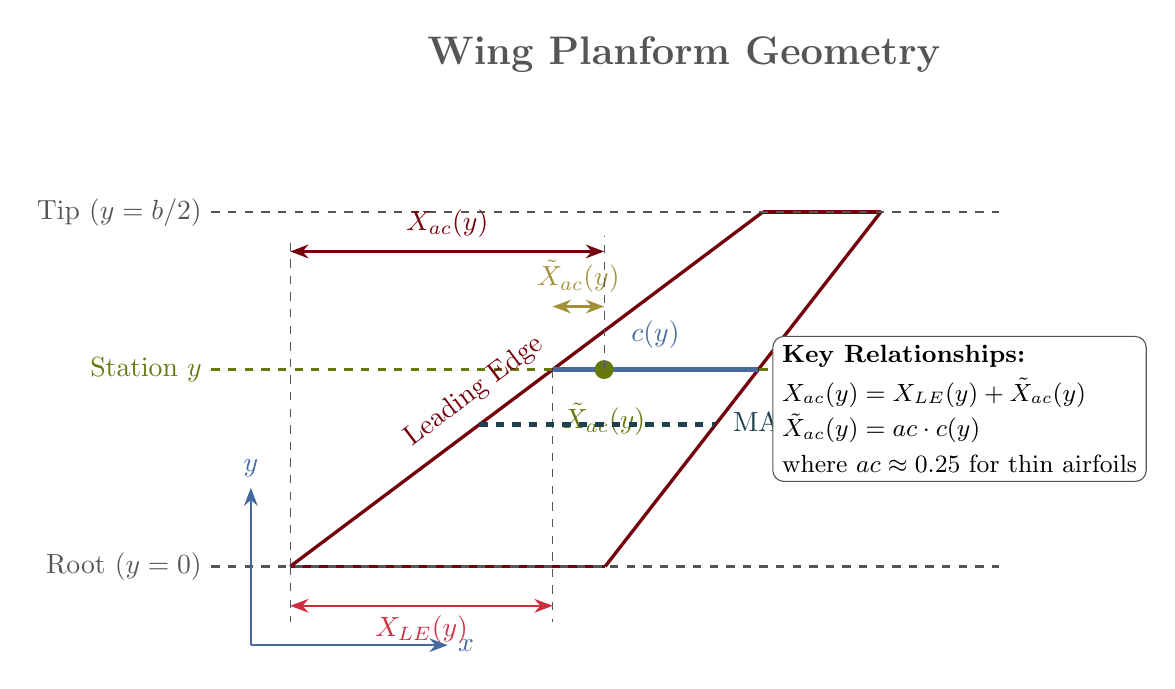
\begin{tikzpicture}[>=Stealth, scale=1.0]
    % Title
    \node[font=\Large\bfseries, USC_Black90] at (5,6.5) {Wing Planform Geometry};

    % Wing planform (swept wing, right semi-span only)
    % Leading edge
    \draw[very thick, Garnet] (0,0) -- (6,4.5);
    % Trailing edge
    \draw[very thick, Garnet] (4,0) -- (7.5,4.5);
    % Root chord
    \draw[very thick, Garnet] (0,0) -- (4,0);
    % Tip chord
    \draw[very thick, Garnet] (6,4.5) -- (7.5,4.5);

    % Centerline (fuselage)
    \draw[thick, dashed, USC_Black90] (-1,0) -- (9,0);
    \node[USC_Black90, left] at (-1,0) {Root ($y=0$)};

    % Tip line
    \draw[thick, dashed, USC_Black90] (-1,4.5) -- (9,4.5);
    \node[USC_Black90, left] at (-1,4.5) {Tip ($y=b/2$)};

    % Coordinate system
    \draw[->, thick, USC_Blue] (-0.5,-1) -- (2,-1) node[right] {$x$};
    \draw[->, thick, USC_Blue] (-0.5,-1) -- (-0.5,1) node[above] {$y$};

    % Spanwise station y
    \def\ystation{2.5}
    \draw[thick, dashed, USC_Olive] (-1,\ystation) -- (9,\ystation);
    \node[USC_Olive, left] at (-1,\ystation) {Station $y$};

    % At station y, show X_LE(y), local chord, and X_ac(y)
    % Calculate LE position at y=2.5 (linear interpolation)
    \pgfmathsetmacro{\xle}{0 + (6-0)*\ystation/4.5}
    \pgfmathsetmacro{\xte}{4 + (7.5-4)*\ystation/4.5}
    \pgfmathsetmacro{\localchord}{\xte - \xle}
    \pgfmathsetmacro{\xlocalac}{\xle + 0.25*\localchord}

    % Local chord line
    \draw[ultra thick, USC_Blue] (\xle,\ystation) -- (\xte,\ystation);
    \node[USC_Blue, above] at ({(\xle+\xte)/2},\ystation+0.15) {$c(y)$};

    % X_LE(y) dimension
    \draw[<->, thick, USC_Rose] (0,-0.5) -- (\xle,-0.5);
    \node[USC_Rose, below] at (\xle/2,-0.5) {$X_{LE}(y)$};

    % Vertical line from origin down to dimension
    \draw[thin, dashed, USC_Black90] (0,0) -- (0,-0.7);
    \draw[thin, dashed, USC_Black90] (\xle,\ystation) -- (\xle,-0.7);

    % Local aerodynamic center marker
    \fill[USC_Olive] (\xlocalac,\ystation) circle (0.12);
    \node[USC_Olive, below] at (\xlocalac,\ystation-0.3) {$\tilde{X}_{ac}(y)$};

    % X_ac(y) = X_LE(y) + tilde{X}_ac(y) annotation
    \draw[<->, thick, USC_Gold] (\xle,\ystation+0.8) -- (\xlocalac,\ystation+0.8);
    \node[USC_Gold, above] at ({(\xle+\xlocalac)/2},\ystation+0.85) {$\tilde{X}_{ac}(y)$};

    % Total X_ac(y) dimension
    \draw[<->, thick, Garnet] (0,\ystation+1.5) -- (\xlocalac,\ystation+1.5);
    \node[Garnet, above] at (\xlocalac/2,\ystation+1.55) {$X_{ac}(y)$};
    \draw[thin, dashed, USC_Black90] (0,0) -- (0,\ystation+1.7);
    \draw[thin, dashed, USC_Black90] (\xlocalac,\ystation) -- (\xlocalac,\ystation+1.7);

    % Leading edge line label
    \node[Garnet, rotate=37, above] at (2.5,2) {Leading Edge};

    % MAC location (dashed, approximate)
    \pgfmathsetmacro{\ymac}{1.8}
    \pgfmathsetmacro{\xlemac}{0 + (6-0)*\ymac/4.5}
    \pgfmathsetmacro{\xtemac}{4 + (7.5-4)*\ymac/4.5}
    \draw[ultra thick, dashed, USC_Slate] (\xlemac,\ymac) -- (\xtemac,\ymac);
    \node[USC_Slate, right] at (\xtemac+0.1,\ymac) {MAC ($\bar{c}$)};

    % Annotation box
    \node[draw=USC_Black90, fill=white, rounded corners, align=left, font=\small] at (8.5,2) {
        \textbf{Key Relationships:}\\[0.3em]
        $X_{ac}(y) = X_{LE}(y) + \tilde{X}_{ac}(y)$\\[0.2em]
        $\tilde{X}_{ac}(y) = ac \cdot c(y)$\\[0.2em]
        where $ac \approx 0.25$ for thin airfoils
    };

\end{tikzpicture}
\end{document}
